\documentclass[11pt,a4paper]{article}
\usepackage[english]{babel}					% Use english
\usepackage[utf8]{inputenc}					% Caracteres UTF-8
\usepackage{graphicx}						% Imagenes
\usepackage[hidelinks]{hyperref}			% Poner enlaces sin marcarlos en rojo
\usepackage{fancyhdr}						% Modificar encabezados y pies de pagina
\usepackage{float}							% Insertar figuras
\usepackage[textwidth=390pt]{geometry}		% Anchura de la pagina
\usepackage[nottoc]{tocbibind}				% Referencias (no incluir num pagina indice en Indice)
\usepackage{enumitem}						% Permitir enumerate con distintos simbolos
\usepackage[T1]{fontenc}					% Usar textsc en sections
\usepackage{amsmath}						% Símbolos matemáticos
\usepackage{amsfonts}
\usepackage{tikz}
\usetikzlibrary{calc}

% Comando para poner el nombre de la asignatura
\newcommand{\subject}{Optimization}
\newcommand{\autor}{Vladislav Nikolov Vasilev}
\newcommand{\titulo}{Optimization Problem 0}
\newcommand{\subtitulo}{The Fermat point of a set of points}
\newcommand{\masters}{Master in Fundamental Principles of Data Science}

\tikzset{
  dot/.style={circle,inner sep=1pt,fill,scale=1.5,label={$#1$},name=#1}
}

\newcommand{\length}[1]{\lvert#1\rvert}
\newcommand{\polyarea}[1]{\left[#1\right]}


% Configuracion de encabezados y pies de pagina
\pagestyle{fancy}
\lhead{\autor{}}
\rhead{\subject{}}
\lfoot{\masters}
\cfoot{}
\rfoot{\thepage}
\renewcommand{\headrulewidth}{0.4pt}		% Linea cabeza de pagina
\renewcommand{\footrulewidth}{0.4pt}		% Linea pie de pagina

\begin{document}
\pagenumbering{gobble}

% Title page
\begin{titlepage}
  \begin{minipage}{\textwidth}
    \centering
    
\includegraphics[scale=0.25]{img/ub-logo}\\[2cm]
    
    \textsc{\Large \subject\\[0.5cm]}
    \textsc{\uppercase\expandafter{\masters}}\\[1.5cm]
    
    \noindent\rule[-1ex]{\textwidth}{1pt}\\[1.5ex]
    \textsc{{\Huge \titulo\\[0.5ex]}}
    \textsc{{\Large \subtitulo\\}}
    \noindent\rule[-1ex]{\textwidth}{2pt}\\[3.5ex]
  \end{minipage}
  
  \vspace{2cm}
  
  \begin{minipage}{\textwidth}
    \centering
    
    
\includegraphics[scale=0.4]{img/ub-ds-logo}
    \vspace{2cm}
    
    \textbf{Author}\\ {\autor{}}\\[2.5ex]
    \textsc{Faculty of Mathematics and Computer Science}\\
    \vspace{1em}
    \textsc{Academic year 2021-2022}
  \end{minipage}
\end{titlepage}

\pagenumbering{arabic}
\setlength{\parskip}{1em}

\noindent \textbf{Given set of points $y_1, \dots, y_m$ in the plane, find a point $x^*$ whose sum of
weighted distances to the given set of points is minimized. Mathematically, the problem is}

\[
  \min \sum_{i=1}^m w_i \left\Vert x^* - y_i \right\Vert, \quad \text{subject to } x^* \in \mathbb{R}^2,
\]

\noindent \textbf{where $w_1, \dots, w_m$ are given positive real numbers.}

\begin{figure}[H]
  \centering
  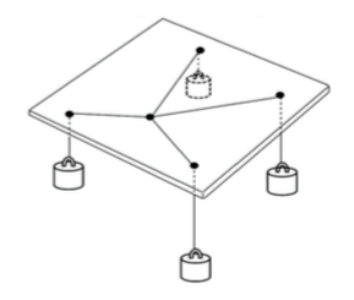
\includegraphics[width=0.4\textwidth]{img/mechanical_system}
  \caption{Example of a mechanical system.}
  \label{fig:mechanical_system}
\end{figure}

\noindent \textbf{1. Show that there exists a global minimum for this problem (that it can be
realized by means of the mechanical model shown in the figure \ref{fig:mechanical_system}).}

Consider the function $f$ defined as $f(x) = \sum_{i=1}^m w_i \left\Vert x - y_i \right\Vert$.
This function is nothing more and nothing less than the weighted sum of the norms
$\left\Vert x - y_i \right\Vert$ for $i = 1, \dots, m$. By definition, any vector norm is
a convex function, and the weighted sum of convex functions is also a convex function provided that
every $w_i$ satisfies that $w_i > 0$ for $i = 1, \dots, m$. This implies that $f$ is convex,
and by definition, a local minimum of $f$ is also a global minimum. Thus, there must exist at least
one $x^*$ such that $x^*$ is a local minimum of the function, and therefore, it is also a global minimum
of the function $f$.

\noindent \textbf{2. Is the optimal solution always unique?}

In this case, the optimal solution is not always unique. Suppose the case in which we have two points
$y_1$ and $y_2$ such that $y_1 \neq y_2$. Also, suppose that the weights are $w_1 = w_2 = 1$. Then
the minimum is attained at all the points
$x^* \in \lbrace \lambda y_1 + (1 - \lambda) \; | \; \lambda \in [0, 1] \rbrace$.
We can see this as follows:

\begin{equation*}
\begin{aligned}
  f(\lambda y_1 + (1 - \lambda)) &= \left\Vert (\lambda - 1) y_1 + (1 - \lambda) y_2 \right\Vert
  + \left\Vert \lambda y_1 - \lambda y_2 \right\Vert = \\
  &= \left\Vert (\lambda - 1) (y_1 - y_2) \right\Vert + \left\Vert \lambda (y_1 - y_2) \right\Vert = \\
  &= (\lambda - 1) \left\Vert y_1 - y_2 \right\Vert + \lambda \left\Vert y_1 - y_2 \right\Vert = \\
  &= \left\Vert y_1 - y_2 \right\Vert
\end{aligned}
\end{equation*}

Therefore, there exist multiple global minima, and the optimal solution is not unique.

\noindent \textbf{3. Show that an optimal solution minimizes the potential energy of the
mechanical model defined as $\sum_{i=1}^m w_i h_i$, where $h_i$ is the height of the ith
weight measured from some reference level.}

Consider the model seen in figure \ref{fig:mechanical_system}. It consists of a platform
with $m$ different massless ropes attached to a point $x^*$ (which in this case is the one
between all of the other points). Each rope goes through one of the $m$, and each
one has attached an object that weights $w_i$ for $i = 1, \dots, m$. The length of
each rope is given by $l_i$, where $l_i \in \mathbb{R}^+$.

Suppose that we set the reference level of the gravitational potential at the platform.
Then, we have that given any attachment point $x$ in the platform, the length of the rope
is given by $l_i = \left\Vert x - y_i \right\Vert + h_i(x)$, for $i = 1, \dots, m$,
where $h_i > 0$ and $-h_i$ is the height of the $i$-th weight measured from the platform.

The potential energy of the physical system can be written as follows:

\begin{equation}
  \label{eq:potential}
  V(x) = - \sum_{i=1}^m w_i h_i (x) = - \sum_{i=1}^m w_i l_i + \sum_{i=1}^m w_i \left\Vert x - y_i \right\Vert = c + f(x)
\end{equation}

\noindent where $c$ is a constant. Therefore, the only way to minimize the result of expression
\eqref{eq:potential} is by minimizing the function $f$.

\end{document}

